\chapter{Introdução}
 Todo engenheiro de computação deve ter conhecimento sobre algoritmos de ordenação, visto que estes estão presentes em diversas aplicações. Este projeto desafia seus participantes a se familiarizarem não só com a implementaçao de tais algoritmos, mas também com seu funcionamento interno, através da analise feita por este relatório.
\section{Objetivo}
  O objetivo deste projeto é comparar o desempenho de diferentes algoritmos de
ordenação em termos de tempo, utilizando uma variedade de
conjuntos de dados.


\chapter{Metodologia}
\section{Preparação}
Para a medição do tempo de execução, primeiro os algorimos foram implementados em python e depois executados nos seguintes grupos de dados:
\begin{itemize}
  \item 10000: ordenados, Inversamente ordenados e aletórios
  \item 20000: ordenados, Inversamente ordenados e aletórios
  \item 40000: ordenados, Inversamente ordenados e aletórios
  \item 80000: ordenados, Inversamente ordenados e aletórios
  \item 100000: ordenados, Inversamente ordenados e aletórios
\end{itemize}

\section{Execução}
Os algoritmos foram exectados um a um através do script \textit{make.sh} com cada um dos dados apresentados na secção \textit{apresentação} e os resultados de tempo gasto, comparações e trocas salvos no arquivo \textit{metrics.txt} que então foram analizados através do notebook jupyter para gerar as figuras e tabelas presentes no relatório.

\section{Reconsiderações}
Durante a execução do projeto, foram feitas as seguintes reconsiderações: 
\begin{itemize}
  \item Os algoritmos foram executados apenas uma vez, por conta da demora de execução dos mesmos. 
  \item As quantidades de comparações e trocas foram medidas para alguns algoritmos, visto que outros (como o count sort) não realizam trocas e nem comparações, por conta disso e da restrição de tempo para entrega, a analise dessas variaveis não foi incluida no relatorio final
  \item A complexidade de espaço não foi medida, visto que a implementação do calculo dessa métrica acarretou no aumento grandioso do já longo tempo de execução dos algoritmos, por isso e pela restrição de tempo, essa métrica não foi nem sequer computada.
\end{itemize}
%%%%%%%%%%%%%%%%%%%%%%%%%%%%%%%%%%%%%%%%%%%%%%%%%%%%%%%%%%%%%%%%%%%%%%%%%%%%%%%%%%%%%%%%%
\chapter{Resultados e Analises}
\section{Resultados para DataSet Ordenado}

\begin{figure}[H]
  \centering
  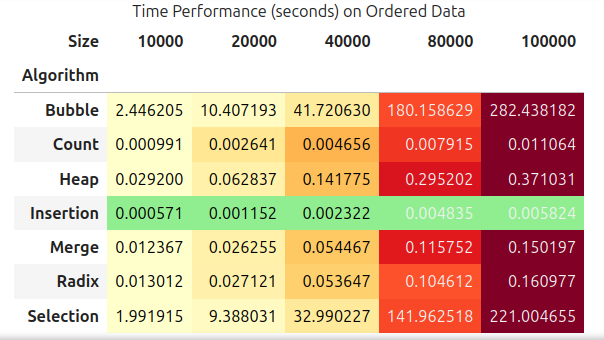
\includegraphics[width=0.6\textwidth]{images/order_table}
  \caption{Tabela Dados Ordeanados}
  \label{fig:Tabela Dados Ordenados}
\end{figure}

\begin{figure}[H]
  \centering
  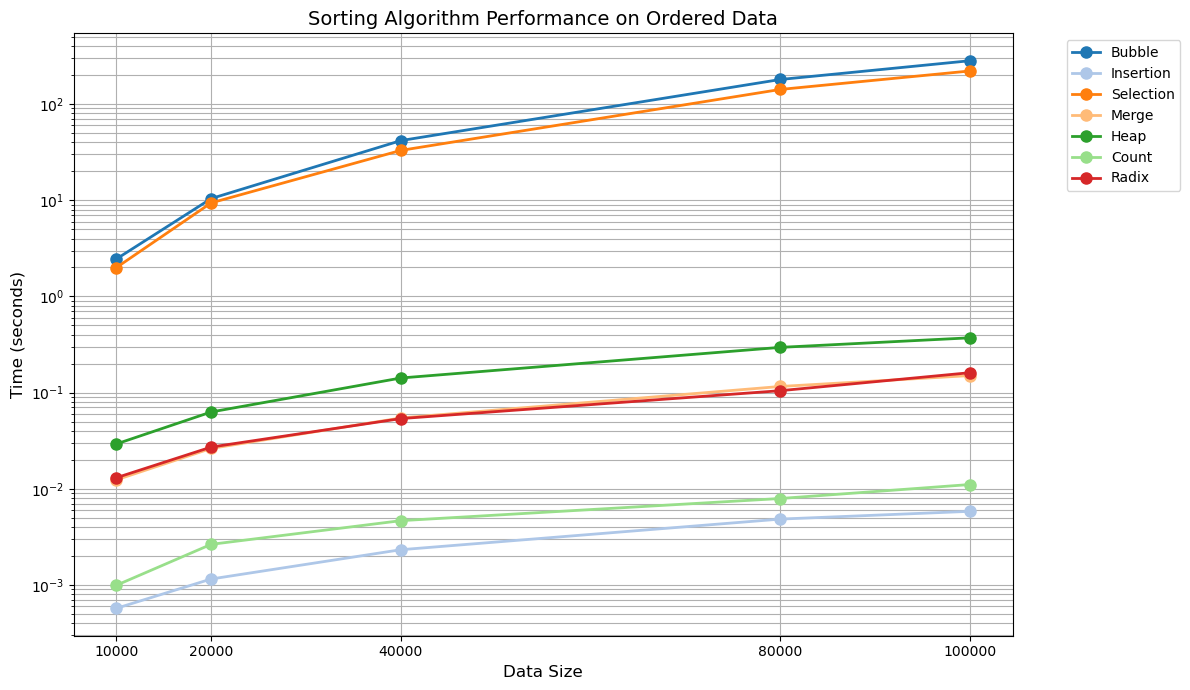
\includegraphics[width=0.6\textwidth]{images/all_algo_order}
  \caption{Gráfico Performance Dados Ordenados em escala Logaritmica}
  \label{fig:Gráfico Performance Dados Ordenados}
\end{figure}

\begin{figure}[H]
  \centering
  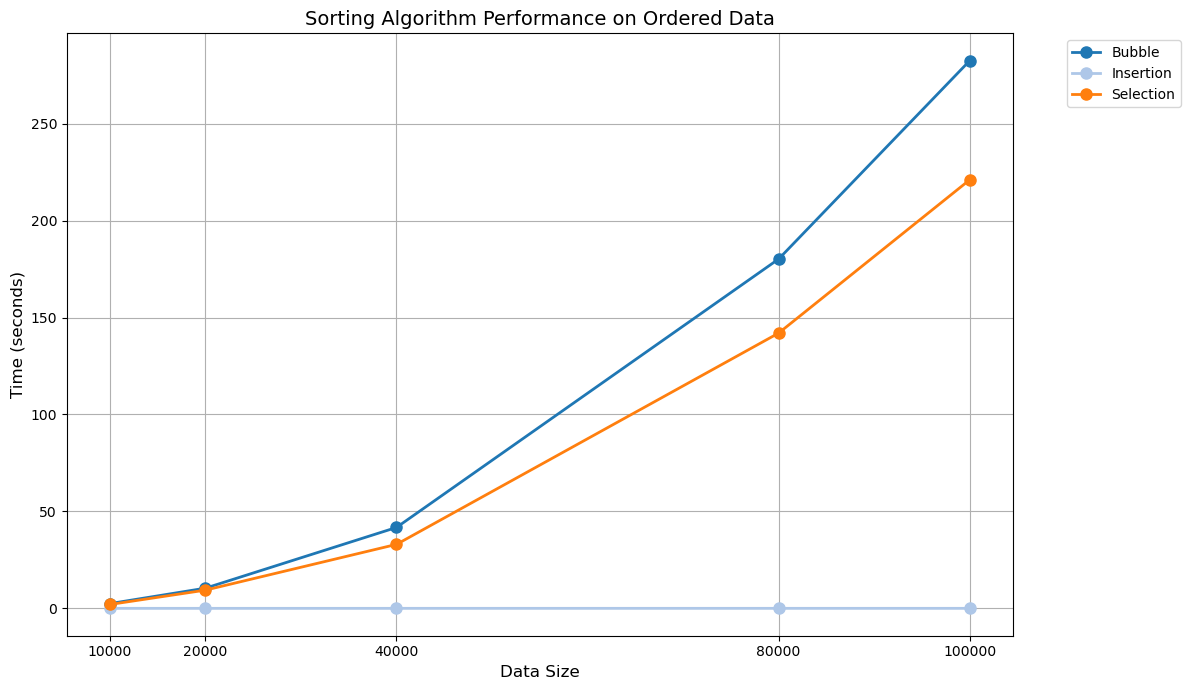
\includegraphics[width=0.6\textwidth]{images/o2_order}
  \caption{Performance Bubble, Insertion e Selection em Dados Ordenados}
  \label{fig:Performance Bubble, Insertion e Selection em Dados Ordenados}
\end{figure}

\begin{figure}[H]
  \centering
  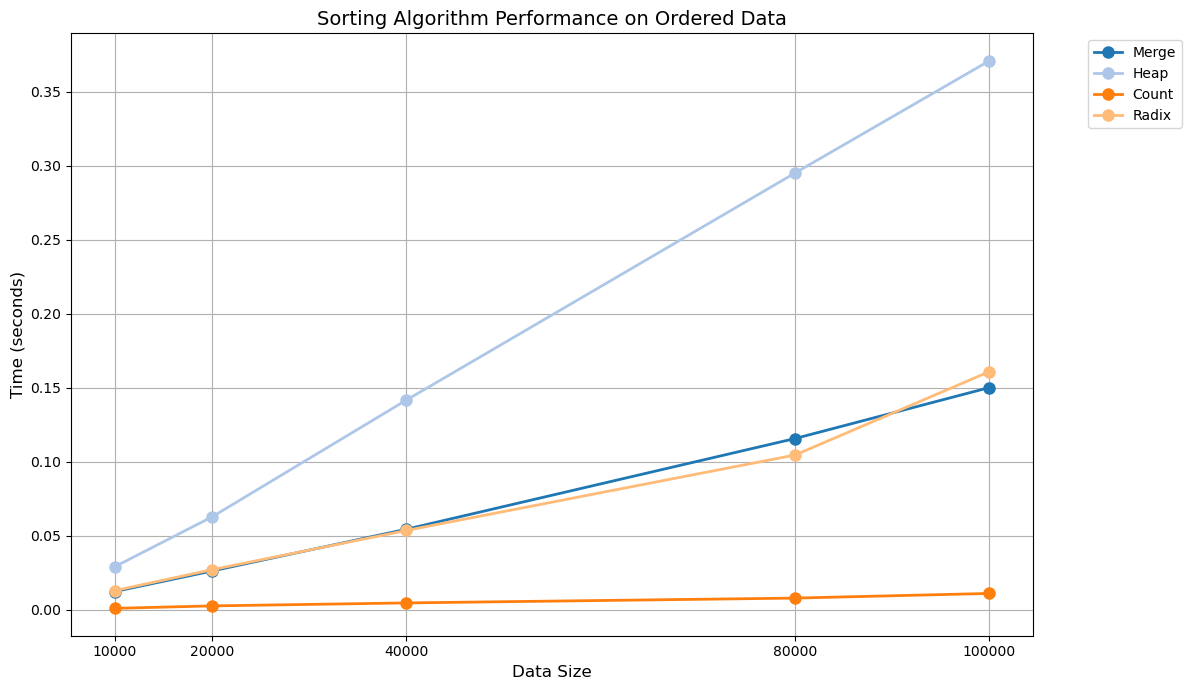
\includegraphics[width=0.6\textwidth]{images/o_order}
  \caption{Performance Restante em Dados Ordenados }
  \label{fig:Gráfico Performance Dados Ordenados}
\end{figure}

\subsection{Analise para Dados Ordenados}
Para os dados Ordenados:
\begin{itemize}
  \item Pior Algorimo: Bubble Sort
  \item Melhor Algoritmo: Insertion Sort
\end{itemize}
Pela analise dos gráficos, observa-se os seguintes comportamentos:
\begin{itemize}
  \item Parabólico: Selection e Bubble. Comportamento esperado 
  \item Logaritmico: Radix e Merge. Esperado para Merge, inesperado para Radix 
  \item Linear: Heap e Insertion. Comportamento Inesperado
\end{itemize}
%%%%%%%%%%%%%%%%%%%%%%%%%%%%%%%%%%%%%%%%%%%%%%%%%%%%%%%%%%%%%%%%%%%%%%%%%%%%%%%%%%%%%%%%%
%%%%%%%%%%%%%%%%%%%%%%%%%%%%%%%%%%%%%%%%%%%%%%%%%%%%%%%%%%%%%%%%%%%%%%%%%%%%%%%%%%%%%%%%%
\section{Resultados para DataSet Inversamente Ordenado}

\begin{figure}[H]
  \centering
  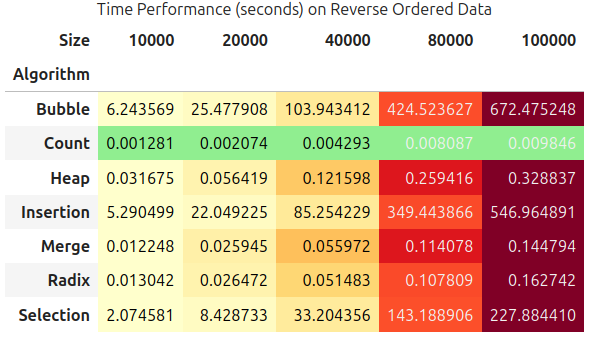
\includegraphics[width=0.6\textwidth]{images/invert_table}
  \caption{Tabela Dados Inversamente Ordenados}
  \label{fig:Tabela Dados Inversamente Ordenados}
\end{figure}

\begin{figure}[H]
  \centering
  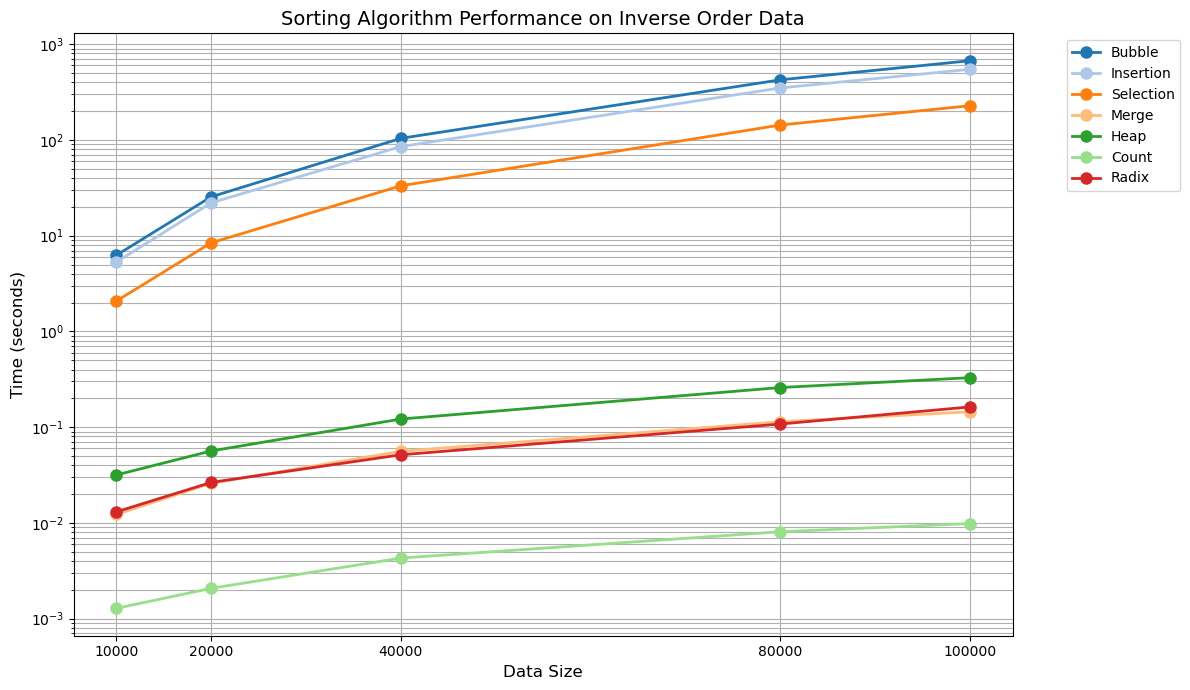
\includegraphics[width=0.6\textwidth]{images/all_algo_inver}
  \caption{Gráfico Performance Dados Inversamente Ordenados em escala Logaritmica}
  \label{fig:Gráfico Performance Dados Inversamente Ordenados}
\end{figure}

\begin{figure}[H]
  \centering
  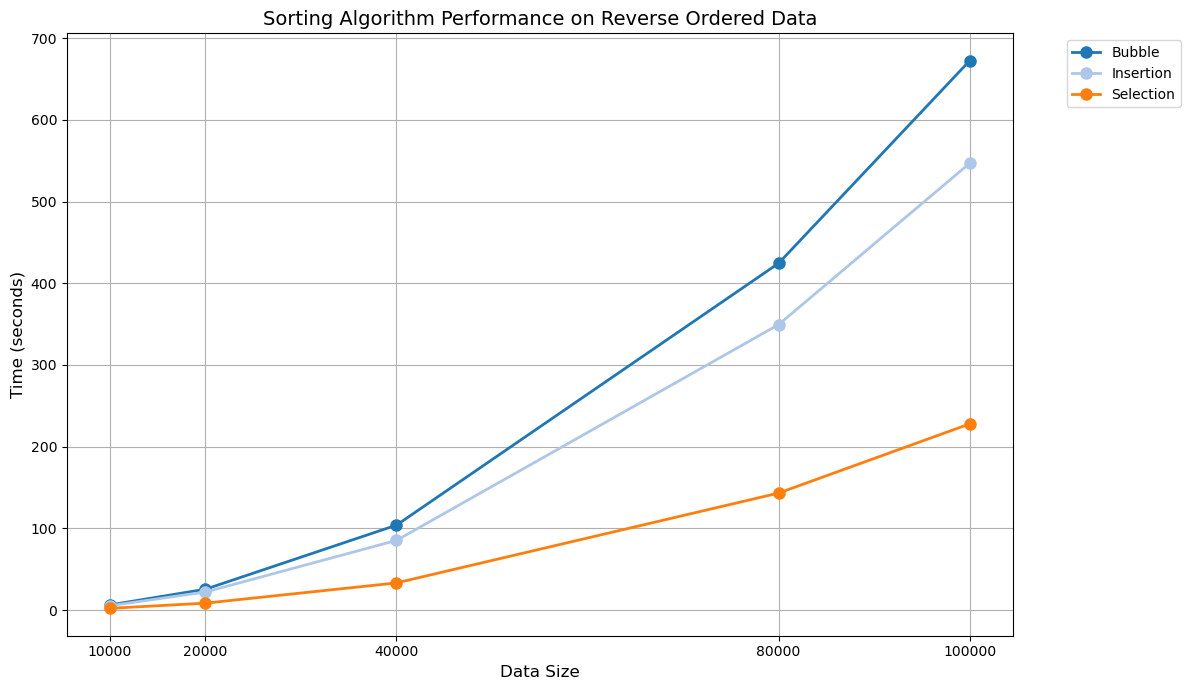
\includegraphics[width=0.6\textwidth]{images/o2_inv}
  \caption{Performance Bubble, Insertion e Selection em Dados Inversamente Ordenados}
  \label{fig:Performance Bubble, Insertion e Selection em Dados Inversamente Ordenados}
\end{figure}

\begin{figure}[H]
  \centering
  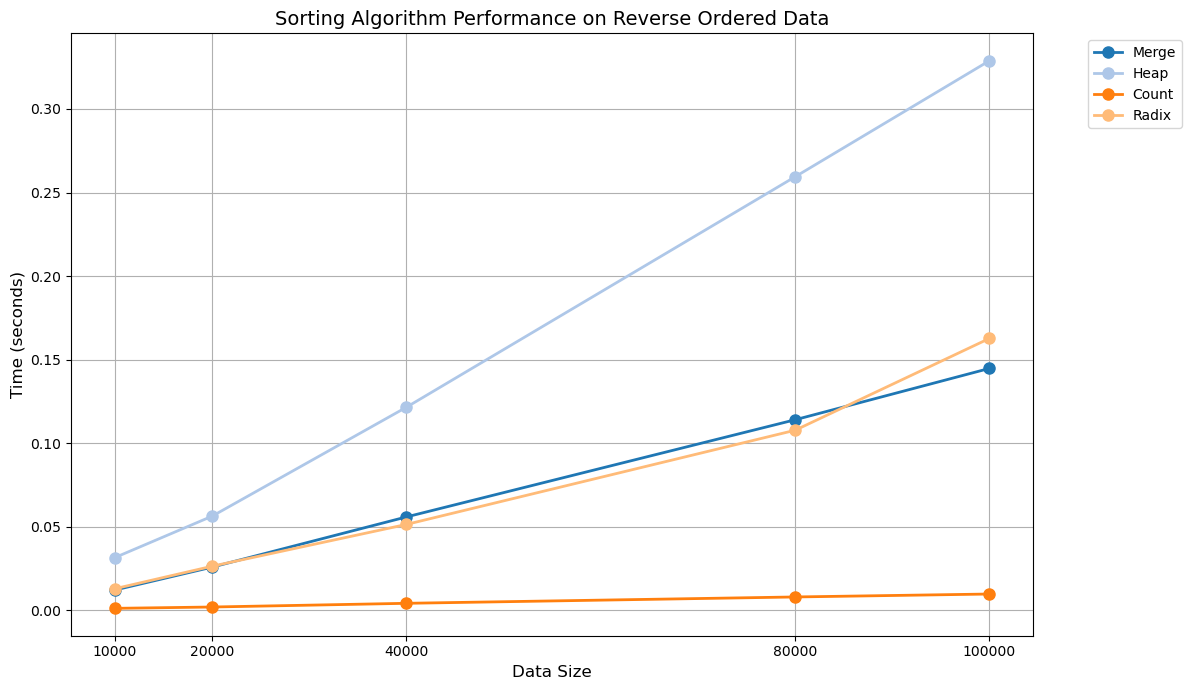
\includegraphics[width=0.6\textwidth]{images/o_inv}
  \caption{Performance Restante em Dados Inversamente Ordenados }
  \label{fig:Gráfico Performance Dados Inversamente Ordenados}
\end{figure}

\subsection{Analise para Dados Inversamente Ordenados}
Para os dados Inversamente Ordenados:
\begin{itemize}
  \item Pior Algorimo: Bubble Sort
  \item Melhor Algoritmo: Count Sort
\end{itemize}
Pela analise dos gráficos, observa-se os seguintes comportamentos:
\begin{itemize}
  \item Parabólico: Selection,  Bubble e Insertion. Comportamento esperado 
  \item Logaritmico: Radix, Merge e Heap. Inesperado para Radix 
  \item Linear: Count. Comportamento Inesperado
\end{itemize}

%%%%%%%%%%%%%%%%%%%%%%%%%%%%%%%%%%%%%%%%%%%%%%%%%%%%%%%%%%%%%%%%%%%%%%%%%%%%%%%%%%%%%%%%%
%%%%%%%%%%%%%%%%%%%%%%%%%%%%%%%%%%%%%%%%%%%%%%%%%%%%%%%%%%%%%%%%%%%%%%%%%%%%%%%%%%%%%%%%%
\section{Resultados para DataSet Aleatoriamente Ordenado}
\begin{figure}[H]
  \centering
  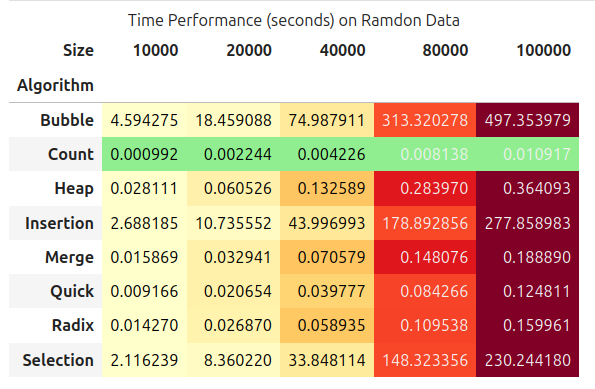
\includegraphics[width=0.6\textwidth]{images/random_table}
  \caption{Tabela Dados Aleatoriamente Ordenados}
  \label{fig:Tabela Dados Aleatoriamente Ordenados}
\end{figure}

\begin{figure}[H]
  \centering
  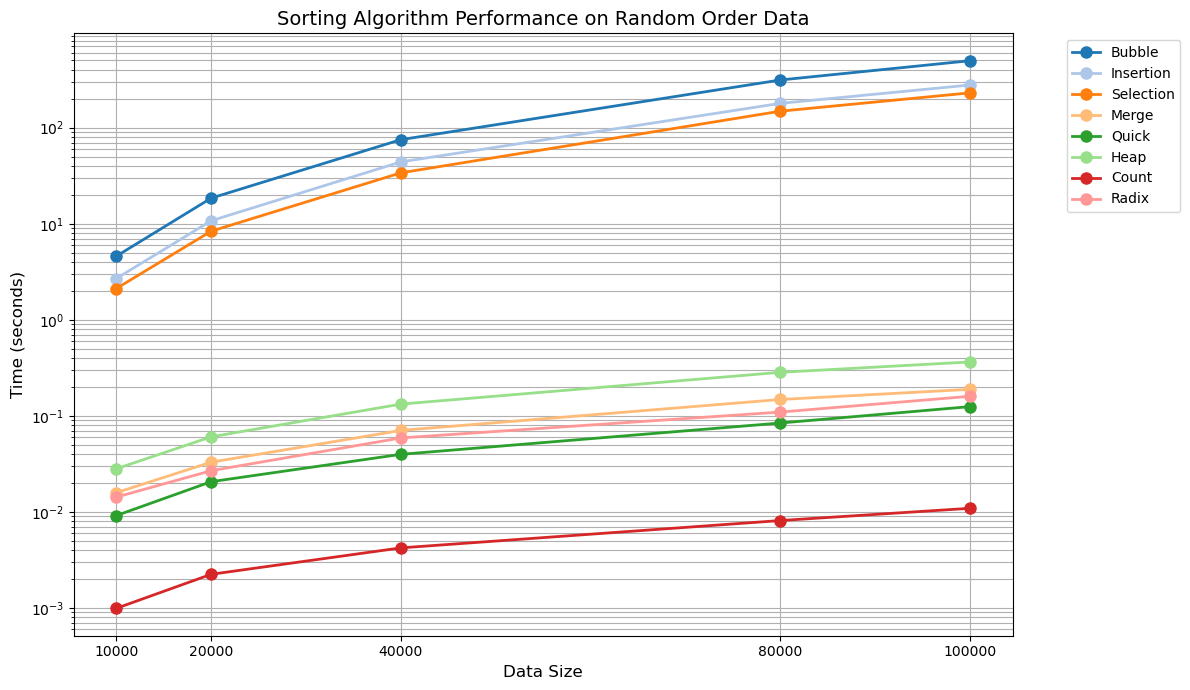
\includegraphics[width=0.6\textwidth]{images/all_algo_rand}
  \caption{Gráfico Performance Dados Aleatoriamente Ordenados em escala Logaritmica}
  \label{fig:Gráfico Performance Dados Aleatoriamente Ordenados}
\end{figure}

\begin{figure}[H]
  \centering
  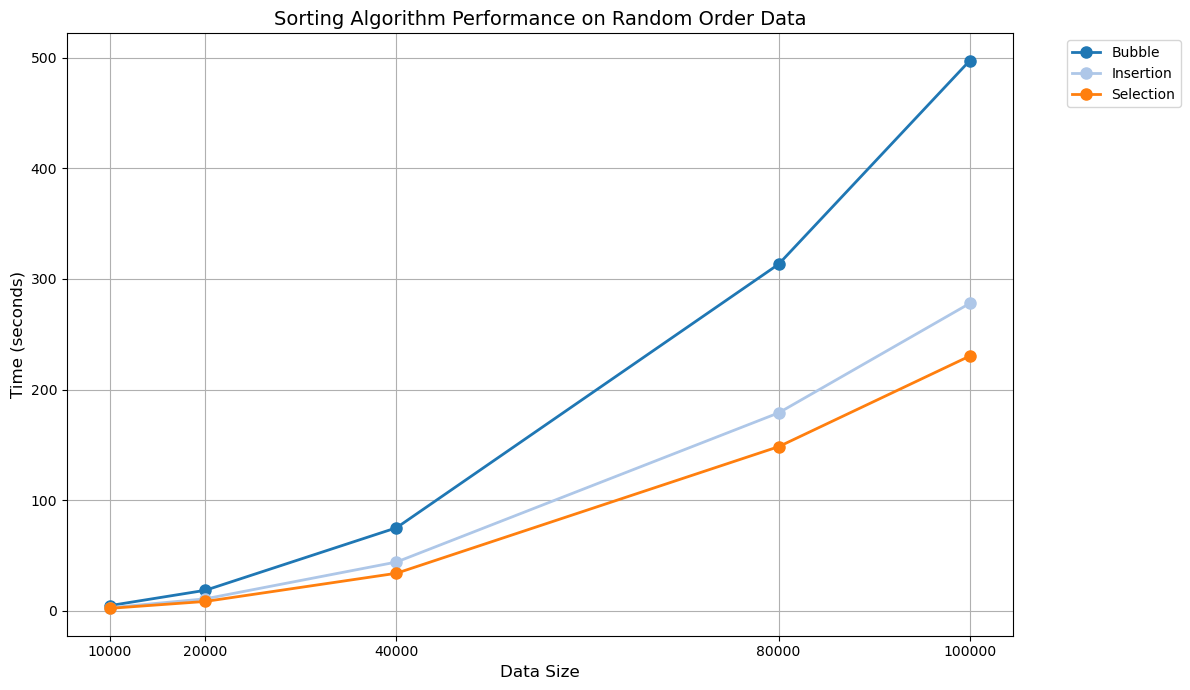
\includegraphics[width=0.6\textwidth]{images/o2_random}
  \caption{Performance Bubble, Insertion e Selection em Dados Aleatoriamente Ordenados}
  \label{fig:Performance Bubble, Insertion e Selection em Dados Aleatoriamente Ordenados}
\end{figure}

\begin{figure}[H]
  \centering
  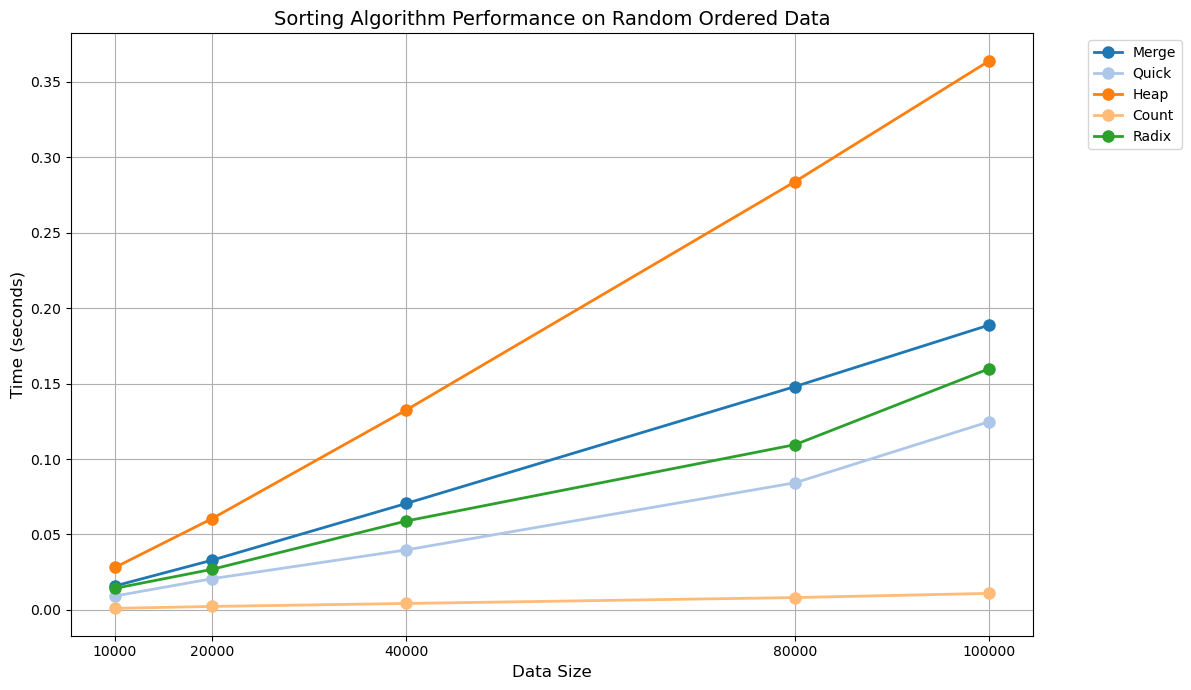
\includegraphics[width=0.6\textwidth]{images/o_random}
  \caption{Performance Restante em Dados Aleatoriamente Ordenados }
  \label{fig:Gráfico Performance Dados Aleatoriamente Ordenados}
\end{figure}

\subsection{Analise para Dados Aleatoriamente Ordenados}
Para os dados Inversamente Aleatoriamente Ordenados:
\begin{itemize}
  \item Pior Algorimo: Bubble Sort
  \item Melhor Algoritmo: Count Sort 
\end{itemize}
Pela analise dos gráficos, observa-se os seguintes comportamentos:
\begin{itemize}
  \item Parabólico: Selection,  Bubble e Insertion. Comportamento esperado 
  \item Logaritmico: Radix, Merge e Quick. Esperado apenas para Merge 
  \item Linear: Count e Heap. Comportamento Inesperado para Heap
\end{itemize}

\chapter{Conclusões}
Um dos comportamentos inesperados para o Radix muito provavelmente vem da implementação do mesmo, que precisa encontrar o máximo dentre os elementos, consequentemente varrendo os mesmos até o final pelo menos uma vez. 
O comportamento dos algotimos também permite concluir que o melhor deles em termos de tempo de execução foi o Counting sort, exceto para o caso dos já ordenados, que foi o Insertion Sort, comportamento esperado do mesmo visto que ele apenas compara uma vez cada elemento, que por conta de estarem na ordem correta não precisam ser comparados com os anteriores, o que acarreta no comportamento linear.

Em conclusão, o projeto permitiu um aprofundamento no conhecimento dos diversos algoritmos de ordenação bem como seu funcionamento interno e requisitos de sistema. 
Uma futura pesquisa poderia pegar a base do projeto porém além de realizar as comparações de tempo dentro da mesma linguagem, realizar a implementação dos memsmos algoritmos em outras linguagens e então comparar o tempo etre elas.

